\documentclass[tikz,border=5pt]{standalone}
\usepackage{tikz}
\usetikzlibrary{shapes.geometric, arrows, 
  positioning,
  shapes.misc   %rounded rectangle
}

% define the tikz style
%Rounded corners only at one side of a TikZ node
\tikzstyle{data} = [fill=gray, rounded rectangle, minimum width=2cm, minimum height=1cm]
\tikzstyle{datawest} = [fill=gray, rounded rectangle, rounded rectangle west arc=none, minimum width=2cm, minimum height=1cm]
\tikzstyle{dataeast} = [fill=yellow, rounded rectangle, rounded rectangle east arc=none, minimum width=2cm, minimum height=1cm]

\begin{document}

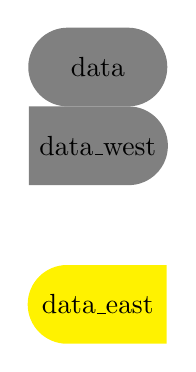
\begin{tikzpicture} [every node]
%\node(id) [style] {text}
  \node (data1) [data]  {data};
  \node (data2) [datawest, below of = data1] {data\_west};
  %"below of = sth" is different with "below = of sth"
  \node (data3) [dataeast, below  = of data2] {data\_east};
\end{tikzpicture}


\begin{tikzpicture}[every node/.style={fill=gray, rounded rectangle, minimum width=2cm, minimum height=1cm}]
    \node [](A){};
    \node [rounded rectangle west arc=none, below=of A](B){};
    \node [rounded rectangle east arc=none, below=of B]{};
\end{tikzpicture}

\end{document}
